\documentclass[coloremph,lightbackground,landscape,a4,17pt]{foils}
\usepackage{times}
\usepackage{color}
\usepackage{fixseminar}
\usepackage{graphics}
\usepackage{hyperref}
\usepackage[display]{texpower}
\usepackage{stepitem}
\usepackage{comment}

\setlength{\voffset}{-1cm}
\addtolength{\textheight}{2cm}

\addtolength{\hoffset}{-1cm}
\addtolength{\textwidth}{2cm}

\begin{document}
\definecolor{gray}{rgb}{.6,.6,.6}
\definecolor{darkblue}{rgb}{0,0,.5}
\definecolor{darkgreen}{rgb}{0,.5,0}
\definecolor{cornsilk}{rgb}{1,.97255,.862745}
\definecolor{moccasin}{rgb}{1,.8941176,.70980392}
\definecolor{khaki}{rgb}{0.941176,0.901961,0.549020}
%\pagecolor{cornsilk}
\pagecolor{khaki}
\newcommand{\newslide}[1]{\newpage\begin{center}%
\color{darkblue}{\large\bf #1}\end{center}}



\title{Representing Numbers}

\begin{comment}
  
The idea here is to talk about how we represent numbers on a computer.
We want to talk about the different possibilities and understand the
different trade-offs (e.g. infinite precision versus finite, fast
representation.)  We want to tie this to how the computer works,
specifically the CPU pipeline discussed in the previous lecture and
this leads us to using the IEEE representation, with its limitations.


We start with bits and then move onto integers and discuss infinite precision.
\end{comment}


\newslide{Representing Numbers on a Computer}
\liststepwise*[\let\hidestepcontents=\displaystepcontents]{%
  \begin{stepitemize}
    \item Representing numbers in a computer involves constraints:
      \begin{itemize}
      \item real numbers must be approximated
      \item integers must be within certain range
      \end{itemize}

    \item  Arithmetic on integers can lead to erroneous results on a
    computer \\ 
     must work within the appropriate precision

    \item Testing for equality of two real numbers is not
      well-defined. \\
       actually comparing approximations \\
       so check for difference smaller than $\epsilon_m$.
  
    \item Can get ``infinite'' precision, but loss in 
     speed and memory utilization.
  \end{stepitemize}
}

\newslide{Bits \& Bytes}
\liststepwise*[\let\hidestepcontents=\displaystepcontents]{%
\begin{stepitemize}
\item Each bit in memory is either on or off: 1 or 0.
\item Represent characters - letters, digits,% +, -, \!, $\ldots$
\item How many different elements?  $128 = 2^7$
\item Use 8 bits to make up a BYTE
\end{stepitemize}
}


\newslide{Representing Integers}
\liststepwise*[\let\hidestepcontents=\displaystepcontents]{%
\begin{stepitemize}
\item How do we represent the following numbers
\item   12351347983413
\item   123513479834131
\item   1235134798341311
\end{stepitemize}
}

\newslide{Possible Approach}
\liststepwise*[\let\hidestepcontents=\displaystepcontents]{%
\begin{stepitemize}
\item Record the collection of digits \\
 \texttt{\{14, \{1, 2, 3, 5, 1, 3, 4, 7, 9, 8, 3, 4, 1, 3\}\}}
\item How do we do calculations? \\
   12351347983413 + 932 \\
\{14, \{1, 2, 3, 5, 1, 3, 4, 7, 9, 8, 3, 4, 1, 3\}\} \\
      + \\
  \{3, \{9, 3, 2\}\} \\
\item Iterate over the digits (in reverse order) \\
      add each digit \\
      record value, carry term
\item Addition of digits done by CPU
\item Iteration done in software \\
      Much slower
\item Need to handle $\infty$, $-\infty$ specially.
\end{stepitemize}
}


\newslide{IEEE Representation}
\liststepwise*[\let\hidestepcontents=\displaystepcontents]{
\begin{stepitemize}
\item Use a restricted representation\\
      use fixed number of bits .
\item Say, 4 bytes = 32 bits.
\item Do arithmetic directly on the chip. \\
    Comparatively, very fast.

\item What is the representation ?

\item Use base 2, i.e. binary

\item  $8 = 2^3 \Rightarrow 1000$
\item  $25 = 2^4 + 2^3 + 2^0 \Rightarrow 11001$

\item $\hbox{value} = \Sigma_{i=0}^{31} x_i 2^i$

\item $i^{th}$ bit in the number indicates whether to include
     $2^i$ in the answer.
  
\end{stepitemize}
}

\newslide{
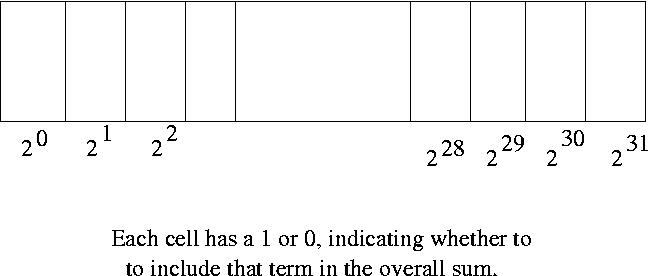
\includegraphics{bit.jpg}

The order in which we organize the bits
(i.e. from left to right or right to left)
is just a convention, and each type of
hardware can do it differently.


% Added after the lecture was given in Davis.
See the bits() function in the R package \RPackage{Rbits}
}




\newslide{Limitations}
\liststepwise*[\let\hidestepcontents=\displaystepcontents]{%

\begin{stepitemize}
 \item Only a finite number of possible values \\
   $-2147483648 (= -2^{31}$) to  $2147483647$ \\
   00000000000000..0000 to 1111111111...11111

\item What happens if we add 1 to $2147483647$?

Get $-2^31$!

\item \texttt{R>  as.integer(2147483647) + as.integer(1)}

Get NA

\item \texttt{R> b = as.integer(1000)} \\
 \texttt{R> b * b * b *b } 

Get NA

\item What about Matlab?
   Stores values as real values \\
   no integers.

\end{stepitemize}
}

\newslide{
\begin{itemize}
  \item Moral: be careful when dealing with integer arithmetic \\
  \item   Know the limitations \\
  \item  Verify results \\
  \item  High-level software will do some checks for you \\
    low-level languages may not.
\end{itemize}
}


\newslide{Real Numbers}
\liststepwise*[\let\hidestepcontents=\displaystepcontents]{%
\begin{stepitemize}
\item  Can we represent arbitrary real numbers?
\item  Use infinite precision approach?
\item  Use fixed point ? \\
        Fixed number of digits after decimal point
\item Is 6/1000 $<$ 14/1000 ? \\
      With 2 decimal places \\
      .01 versus .01 

\item Unnecessary precision for large numbers

\item  Scientific Notation

\item  $6 x 10^-3$  $<$ $1.4x 10^-2$

\item  4 elements:
  \begin{itemize}
  \item sign
  \item exponent
  \item mantissa
  \item base
  \end{itemize}

\item  1 $\le$ mantissa $<$ base \\
     yields unique representation \\
     $6x10^-3$, not $60 x 10^4$

\item For decimal, base $= 10$.
\item For computers, base $= 2$.
\end{stepitemize}
}

\newslide{Representation in a computer}
\liststepwise*[\let\hidestepcontents=\displaystepcontents]{%
  \begin{stepitemize}
    \item $x  =  (-1)^x_0 (\Sigma_{i=1}^t)*2^k$

    \item k is the \textbf{exponent} \\
       integer
    \item $x_0$ is the sign \\
        1 means negative
    \item For  double precision (8 bytes = 64 bits) \\
           exponent uses 11 bits =  2048 possible values \\
           -1022 to 1024

    \item 64 - (1 + 11) = 52 bits for mantissa.

    \item 21/16 is 1.0101  \\
       1 + no halves + 1 quarter + no eighths + 1 sixteenth
  \end{stepitemize}
}


\newslide{Exponent}
\liststepwise*[\let\hidestepcontents=\displaystepcontents]{%
\begin{stepitemize}

   \item Shift value to give -1022 to 1024 

   \item Where did the other value go?
% used to represent underflow.
   \item Represent 0 as a floating point?  

   \item Represent NaN using an exponent with all 1's

 \end{stepitemize}
}


\newslide{Exercise}
\liststepwise*[\let\hidestepcontents=\displaystepcontents]{%
  \begin{stepitemize}
    \item Represent 1.4 as a floating point.
       

    \item How many representations of 0 do we have?
  \end{stepitemize}
}


\newslide{Real Numbers}
\liststepwise*[\let\hidestepcontents=\displaystepcontents]{%

  \begin{stepitemize}
    \item x is a real number
    \item f(x) = $x^\ast$ is the approximation on the computer.

    \item $\vert x - f(x)\vert \big/\vert x\vert$ is the
    \textit{relative error}

     \item $f(x) = x(1 + d_x)$

  \end{stepitemize}
}


\newslide{Real Numbers}
\liststepwise*[\let\hidestepcontents=\displaystepcontents]{%
  \begin{stepitemize}
    \item \textbf{.Machine} in R gives information about representation.

    \item  What is \texttt{.Machine\$machine.double.eps}?
\texttt{
> .Machine\$double.eps
[1] 2.220446e-16
}

   \item The smallest value when added to $1$ that gives a different number

   \item This is the smallest value that we can use to differentiate
       between to numbers.

   \item Are the floating points uniformly distributed along the real line?

   \item What does this imply about accuracy, relative accuracy?

  \end{stepitemize}
}

\newslide{Real Numbers}
\liststepwise*[\let\hidestepcontents=\displaystepcontents]{%
  \begin{stepitemize}
    \item Adding numbers compounds errors.

    \item $S = x_1 + x_2 + x_3$
    \item $S^\ast = \Sigma f(x) = f(x_1) + f(x_2) + f(x_3)$
    \item $=  f(x_1(1+\delta_1) + x_2(1+\delta_2)) + x_3(1+\delta_3)$
    \item $ = (x_1(1+\delta_1) + x_2(1+\delta_2))(1 + \delta_{x_{1} +
    x_{2}}) + x_3(1 + \delta_3)$
    \item In general,
        $\vert \Sigma x_i - \Sigma f(x) \vert  \le  max \vert x_i
    \vert \epsilon_m (n^2  + 3n  -2)/2$  


    \item As we add more numbers, we \textit{potentially} get a lot of
    error!

    \item Sorting and adding the small ones first can help.

  \end{stepitemize}
}

\newslide{Example in R}{
\begin{verbatim}
x = rnorm(2^18)
> length(x)
[1] 262144
> sum(x)
[1] -85.94895
> 
> 
> sum(sort(x))
[1] -85.94895
> options(digits=16)
> sum(sort(x))
[1] -85.94894880246235
> sum(x)
[1] -85.9489488019606
> 
\end{verbatim}
}

\end{document}
